\documentclass[10pt,a4paper,twocolumn]{article}

\usepackage[T1]{fontenc}
\usepackage[utf8]{inputenc}
\usepackage{amsmath}
\usepackage{newpxtext,newpxmath}
\usepackage[top=2.2cm,bottom=2cm,left=1.6cm,right=1.6cm,columnsep=0.75cm,headsep=0.5cm]{geometry}
\usepackage{graphicx}
\usepackage{booktabs}
\usepackage{caption}
\usepackage{xcolor}
\usepackage[hidelinks]{hyperref}
\usepackage{titlesec}
\usepackage{fancyhdr}

\titleformat{\section}{\large\bfseries}{\thesection}{0.8em}{}
\titleformat{\subsection}{\normalsize\bfseries}{\thesubsection}{0.8em}{}
\titlespacing*{\section}{0pt}{10pt}{4pt}
\titlespacing*{\subsection}{0pt}{7pt}{2pt}
\setlength{\textfloatsep}{9pt plus 2pt minus 2pt}
\setlength{\dbltextfloatsep}{9pt plus 2pt minus 2pt}
\setlength{\intextsep}{8pt plus 2pt minus 2pt}
\setlength{\abovecaptionskip}{4pt}
\captionsetup{font=small,labelfont=bf}
\setlength{\parindent}{1em}
\setlength{\parskip}{0pt}

\pagestyle{fancy}
\fancyhf{}
\fancyhead[L]{\small\color{black!60}Movie rating prediction with Bayesian factorization machines}
\fancyhead[R]{\small\color{black!60}Revillon \& Ami}
\fancyfoot[C]{\small\thepage}
\renewcommand{\headrulewidth}{0.4pt}

\graphicspath{{../figures/}{../figures/analysis_report/}}

\newcommand{\R}{\mathbb{R}}
\newcommand{\E}{\mathbb{E}}
\newcommand{\Var}{\mathrm{Var}}
\newcommand{\Cov}{\mathrm{Cov}}
\newcommand{\N}{\mathcal{N}}
\newcommand{\rhat}{\hat r}

\begin{document}

%% ---------------------------------------------------------------- cover page
\begin{titlepage}
\onecolumn
\centering
\vspace*{3.5cm}
{\color{black!60}Data Science Lab \quad$\cdot$\quad Master IASD \quad$\cdot$\quad Assignment 1\par}
\vspace{1.4cm}
{\LARGE\bfseries Movie rating prediction\\[4pt] with Bayesian factorization machines\par}
\vspace{1.2cm}
{\large Quentin Revillon \qquad Vincent Ami\par}
\vspace{0.3cm}
{\color{black!60}Group 40, \textit{La piscine} \quad$\cdot$\quad October 2026\par}
\vspace{1.6cm}
\begin{minipage}{0.82\linewidth}
\small
\centerline{\bfseries Abstract}
\vspace{4pt}
We predict missing ratings in a $610 \times 4980$ movie rating matrix of which $2\%$ of the entries are
observed. All models are compared on the same five folds of the $63\,196$ ratings that the platform fits on,
with a paired test. Regularized biases reach an RMSE of $0.864$, and matrix factorization and neighbourhood
models improve on them by at most $0.012$. Averaging over the posterior (BPMF) gains $0.007$ over the same
factorization fitted by gradient descent, and a Bayesian factorization machine with the corrected genres and
implicit feedback reaches $0.817$; the average of five chains gives $0.812$. An error analysis shows that the
shrinkage of extreme ratings towards the mean is what RMSE requires, that a per-user normalization corrects
the users whose ratings are spread out ($0.805$), and that rarely rated movies remain the hardest case. A
linear stack with an item kNN and a gradient-boosted correction bring the final model to $0.802$.
\end{minipage}
\vspace{1.2cm}

\begin{minipage}{0.6\linewidth}
\small
\setcounter{tocdepth}{1}
\renewcommand{\contentsname}{\normalsize Contents}
\tableofcontents
\end{minipage}
\vspace*{\fill}
\end{titlepage}
\twocolumn
\setcounter{page}{1}

%% ================================================================ 1
\section{Problem, data and protocol}

The ratings form a matrix $R \in \R^{n_u \times n_i}$ with $n_u = 610$ users and $n_i = 4980$ movies,
ratings in $\{0.5, 1, \dots, 5\}$. $\Omega$ is the set of observed pairs $(u,i)$, $\Omega_u$ the movies
rated by $u$ and $\Omega_i$ the users who rated $i$. Train and test each hold $31\,598$ ratings, $1.04\%$ of
the entries. A model outputs $\rhat_{ui}$ for every pair and is scored by
\[
\mathrm{RMSE} = \Big(\frac{1}{|\Omega_{\text{eval}}|}\sum_{(u,i)\in\Omega_{\text{eval}}} (r_{ui}-\rhat_{ui})^2\Big)^{1/2}.
\]
All predictions are clipped to $[0.5, 5]$.

The platform fits our model on train $\cup$ test, so we cross-validate on that union: its $63\,196$ ratings
are split at random into five folds, and each model is fitted on four folds (about $50\,600$ ratings) and
scored on the fifth. Evaluating close to the platform's input size matters, because the best settings depend
on the amount of data (Section~\ref{sec:fm-results}). Hyperparameters were chosen beforehand by 5-fold
cross-validation on the train set alone, except the rank and the number of iterations of the factorization
machine, chosen on the folds of the union.

All models see the same folds, so we compare them fold by fold. The training sets of two folds share three
quarters of their ratings, so the five differences are correlated and a plain $t$-test would be overconfident.
We report the number of folds on which a model wins and the corrected resampled $t$-test of Nadeau and
Bengio~\cite{nadeau}. On the platform, the score has stayed about $0.009$ below our CV score, as the platform
model sees $25\%$ more ratings than a fold.

Besides NumPy and SciPy, we used \texttt{myfm}~\cite{myfm} (Gibbs sampler of the Bayesian factorization
machine), scikit-learn (gradient boosting) and Optuna (hyperparameter search).

%% ================================================================ 2
\section{Building the baseline}

\subsection{Rating biases}
The model $\rhat_{ui} = \mu + b_u + b_i$, where $\mu$ is the mean rating, solves
\[
\min_{b} \sum_{(u,i)\in\Omega} (r_{ui} - \mu - b_u - b_i)^2 + \lambda_u \lVert b_u\rVert^2 + \lambda_i \lVert b_i\rVert^2
\]
by alternating exact ridge updates, e.g.\ $b_i = \sum_{u\in\Omega_i}(r_{ui}-\mu-b_u)/(\lambda_i+|\Omega_i|)$.
Cross-validation gives $\lambda_u = 5$ and $\lambda_i = 3$, so the bias of a movie rated once is divided by 4.
The regularization lowers the RMSE from $0.8844$ to $0.8642$ (Table~\ref{tab:all}).

\subsection{Matrix factorization}
We add a low-rank interaction, $\rhat_{ui} = \mu + b_u + b_i + \langle U_u, V_i\rangle$ with
$U \in \R^{n_u\times k}$ and $V \in \R^{n_i\times k}$ (the course writes $R \approx U I^\top$), and minimize
the squared error plus
\[
\lambda_U\lVert U\rVert^2 + \lambda_V\lVert V\rVert^2 + \lambda_b(\lVert b_u\rVert^2+\lVert b_i\rVert^2).
\]
We compared full-batch gradient descent with momentum and ALS, whose steps are row-wise ridge regressions.
On the same cost, ALS reaches the same validation RMSE as gradient descent about five times faster (3.4\,s
against 17\,s). The model without $\mu$ and biases, $\rhat_{ui} = \langle U_u, V_i\rangle$, is much worse than
the biases ($0.9405$): a rank-$k$ model has to spend its capacity on the mean levels. An Optuna search on the
train set (30 trials, separate $\lambda_U, \lambda_V, \lambda_b$) drives $\lambda_U$ to $54$ and the rank to 2,
which switches the factors off ($0.8632$). With rank 50 and $\lambda = 10$, the factorization gains $0.009$ over
the biases, on every fold.

\subsection{Neighbourhood models}
The item kNN corrects the bias residuals $e_{uj} = r_{uj} - \mu - b_u - b_j$:
\begin{gather*}
\rhat_{ui} = \mu + b_u + b_i + \frac{\sum_{j \in N_k(i;u)} s_{ij}\, e_{uj}}{\delta + \sum_{j\in N_k(i;u)} |s_{ij}|},\\
s_{ij} = \frac{n_{ij}}{n_{ij}+\beta}\,\rho_{ij},
\end{gather*}
where $N_k(i;u)$ are the $k = 20$ movies rated by $u$ most similar to $i$, $\rho_{ij}$ is the Pearson
correlation of the residuals over the $n_{ij}$ common users, $\beta = 100$ shrinks similarities computed on
few users and $\delta = 0.5$ damps the correction when the neighbours are weak. We also tried the user kNN
and Koren's global neighbourhood model~\cite{koren}, where the weights $w_{ij}$ are learnt instead of set to
$s_{ij}$.

\subsection{Results}
Every method of the course beats the biases on every fold, but by at most $0.012$ (item kNN,
Table~\ref{tab:all}). At this density, a movie has 3 training ratings on median in the train set and 6 in
the union: the user and movie offsets are well estimated, the interaction term is not. Point estimates of
$U$ and $V$ either overfit or, once regularized enough, shrink towards zero, and a neighbourhood needs many
common raters to be trusted. We keep $\mu + b_u + b_i$ as the baseline that every model must beat.

\begin{table*}[t]
\centering\small
\setlength{\tabcolsep}{4.5pt}
\begin{tabular}{@{}llcclcc@{}}
\toprule
 & Model & CV RMSE & Gain & relative to & Folds & $p$ \\
\midrule
Baselines     & Global mean                                   & 1.0347 &           &                    &     &        \\
              & Biases, no regularization                     & 0.8844 &           &                    &     &        \\
              & Biases, $\lambda_u=5$, $\lambda_i=3$          & 0.8642 & $-0.0202$ & no regularization  & 5/5 & 0.001  \\
\midrule
Factorization & On raw ratings, gradient descent ($k=2$)      & 0.9405 &           &                    &     &        \\
              & With biases, ALS + Optuna ($k=2$)             & 0.8632 & $-0.0010$ & biases             & 5/5 & $<0.001$ \\
              & With biases, gradient descent ($k=50$, $\lambda=10$) & 0.8553 & $-0.0090$ & biases      & 5/5 & $<0.001$ \\
\midrule
Neighbours    & User kNN ($k=40$)                             & 0.8570 & $-0.0072$ & biases             & 5/5 & $<0.001$ \\
              & Item kNN ($k=20$, $\beta=100$, $\delta=0.5$)  & 0.8523 & $-0.0119$ & biases             & 5/5 & $<0.001$ \\
              & Koren, learnt weights ($k=200$)               & 0.8538 & $-0.0105$ & biases             & 5/5 & $<0.001$ \\
\midrule
BPMF          & $\alpha = 2$ (paper)                          & 0.8505 & $-0.0137$ & biases             & 5/5 & 0.003  \\
(rank 10)     & $\alpha = 1.5$                                & 0.8479 & $-0.0073$ & gradient descent   & 5/5 & 0.006  \\
              & $\alpha$ sampled                              & 0.8493 & $+0.0014$ & $\alpha = 1.5$     & 1/5 & 0.32   \\
\midrule
Bayesian FM   & No features                                   & 0.8465 &           &                    &     &        \\
(rank 20)     & + implicit feedback                           & 0.8340 & $-0.0125$ & no features        & 5/5 & $<0.001$ \\
              & + genres                                      & 0.8190 & $-0.0275$ & no features        & 5/5 & $<0.001$ \\
              & + implicit feedback and genres                & 0.8171 & $-0.0019$ & genres             & 4/5 & 0.17   \\
              & \quad same, first genre file                  & 0.8332 & $+0.0162$ & corrected file     & 0/5 & $<0.001$ \\
\midrule
Ensembles     & FM, average of 5 chains                       & 0.8117 & $-0.0054$ & 1 chain            & 5/5 & 0.003  \\
              & \quad + item kNN, linear stack (submission 3) & 0.8098 & $-0.0019$ & 5 chains           & 5/5 & 0.002  \\
              & FM on user-normalized ratings, 5 chains       & 0.8049 & $-0.0068$ & raw ratings        & 5/5 & $<0.001$ \\
              & \quad + item kNN, linear stack                & 0.8048 & $-0.0001$ & normalized FM      & 3/5 & 0.61   \\
              & \quad + raw FM, item kNN, boosting (final)    & \textbf{0.8023} & $-0.0025$ & linear stack & 5/5 & 0.002  \\
\bottomrule
\end{tabular}
\caption{Every model on the same five folds of train $\cup$ test. Gain: mean decrease of the RMSE relative
to the model in the next column. Folds: folds on which the model is better. $p$: corrected resampled $t$-test.
The fold-to-fold standard deviation of the RMSE is about $0.004$. Submission 3 scored $0.801$ on the platform.}
\label{tab:all}
\end{table*}

%% ================================================================ 3
\section{Bayesian probabilistic matrix factorization}

Salakhutdinov and Mnih~\cite{bpmf} replace the point estimate of $(U, V)$ by an average over the posterior,
which integrates the regularization instead of tuning it. We use the variant with biases, where the bias is
appended to each latent vector, $U_u \leftarrow (U_u, b_u)$ and $V_i \leftarrow (V_i, b_i)$, of dimension
$D = k + 1$.

The likelihood, priors and hyperpriors are
\begin{gather*}
r_{ui} \mid U, V \sim \N\!\big(\mu + \langle U_u, V_i\rangle,\ \alpha^{-1}\big),\\
U_u \mid \mu_U, \Lambda_U \sim \N(\mu_U, \Lambda_U^{-1}),\\
V_i \mid \mu_V, \Lambda_V \sim \N(\mu_V, \Lambda_V^{-1}),\\
p(\mu_U, \Lambda_U) = \N\!\big(\mu_U \mid \mu_0, (\beta_0\Lambda_U)^{-1}\big)\\
\times\mathcal{W}(\Lambda_U \mid W_0, \nu_0),
\end{gather*}
and the same for $(\mu_V, \Lambda_V)$, with the paper's values $\mu_0 = 0$, $\beta_0 = 2$, $W_0 = I_D$,
$\nu_0 = D$. The noise precision $\alpha$ is the only fixed hyperparameter; $\alpha^{-1/2}$ is the standard
deviation of a rating around the model.

\subsection{Gibbs sampling}
The Gauss-Wishart prior is conjugate, so every block has a closed-form conditional posterior. Given $U$, with
mean $\bar U$ and empirical covariance $\bar S$ over its $n_u$ rows, $(\mu_U, \Lambda_U)$ is Gauss-Wishart with
\begin{gather*}
\beta^* = \beta_0 + n_u,\qquad \nu^* = \nu_0 + n_u,\\
\mu^* = \frac{\beta_0\mu_0 + n_u\bar U}{\beta_0 + n_u},\\
\begin{aligned}
(W^*)^{-1} = W_0^{-1} &+ n_u\bar S\\
&+ \frac{\beta_0 n_u}{\beta_0+n_u}(\mu_0-\bar U)(\mu_0-\bar U)^\top .
\end{aligned}
\end{gather*}
Given $V$ and the hyperparameters, the users are independent Gaussians,
$U_u \mid \cdot \sim \N\!\big(m_u, A_u^{-1}\big)$ with
\begin{gather*}
A_u = \Lambda_U + \alpha\!\sum_{i\in\Omega_u}\! V_i V_i^\top,\\
m_u = A_u^{-1}\Big(\Lambda_U\mu_U + \alpha\!\sum_{i\in\Omega_u}\!(r_{ui}-\mu)\,V_i\Big).
\end{gather*}
The mean $m_u$ is a ridge regression of the user's ratings on the movie vectors, with the learnt prior
$(\mu_U, \Lambda_U)$ in place of a hand-tuned $\lambda$; the movies are symmetric. One Gibbs iteration draws
$(\mu_U,\Lambda_U)$, then all $U_u$, then $(\mu_V,\Lambda_V)$ and all $V_i$. After a burn-in of 20
iterations, the prediction is the average of the samples' predictions,
\[
\rhat_{ui} = \frac{1}{T}\sum_{t=1}^{T}\big(\mu + \langle U^{(t)}_u, V^{(t)}_i\rangle\big),
\]
a Monte Carlo estimate of the posterior mean. The chain starts from a few ALS iterations, as the paper starts
from the MAP solution; 2, 10 or 30 of them give the same CV RMSE within $0.003$.

\subsection{Results}
The averaging is what makes the model work. On the validation folds, the RMSE of a single sample rises from
$0.90$ to $0.92$ as the chain explores, while the RMSE of the running average decreases to $0.848$: each
sample overfits, their average does not. With the same model and the same data, the posterior mean gains
$0.007$ over the factorization fitted by gradient descent, on every fold (Table~\ref{tab:all}).

\begin{figure}[t]
\centering
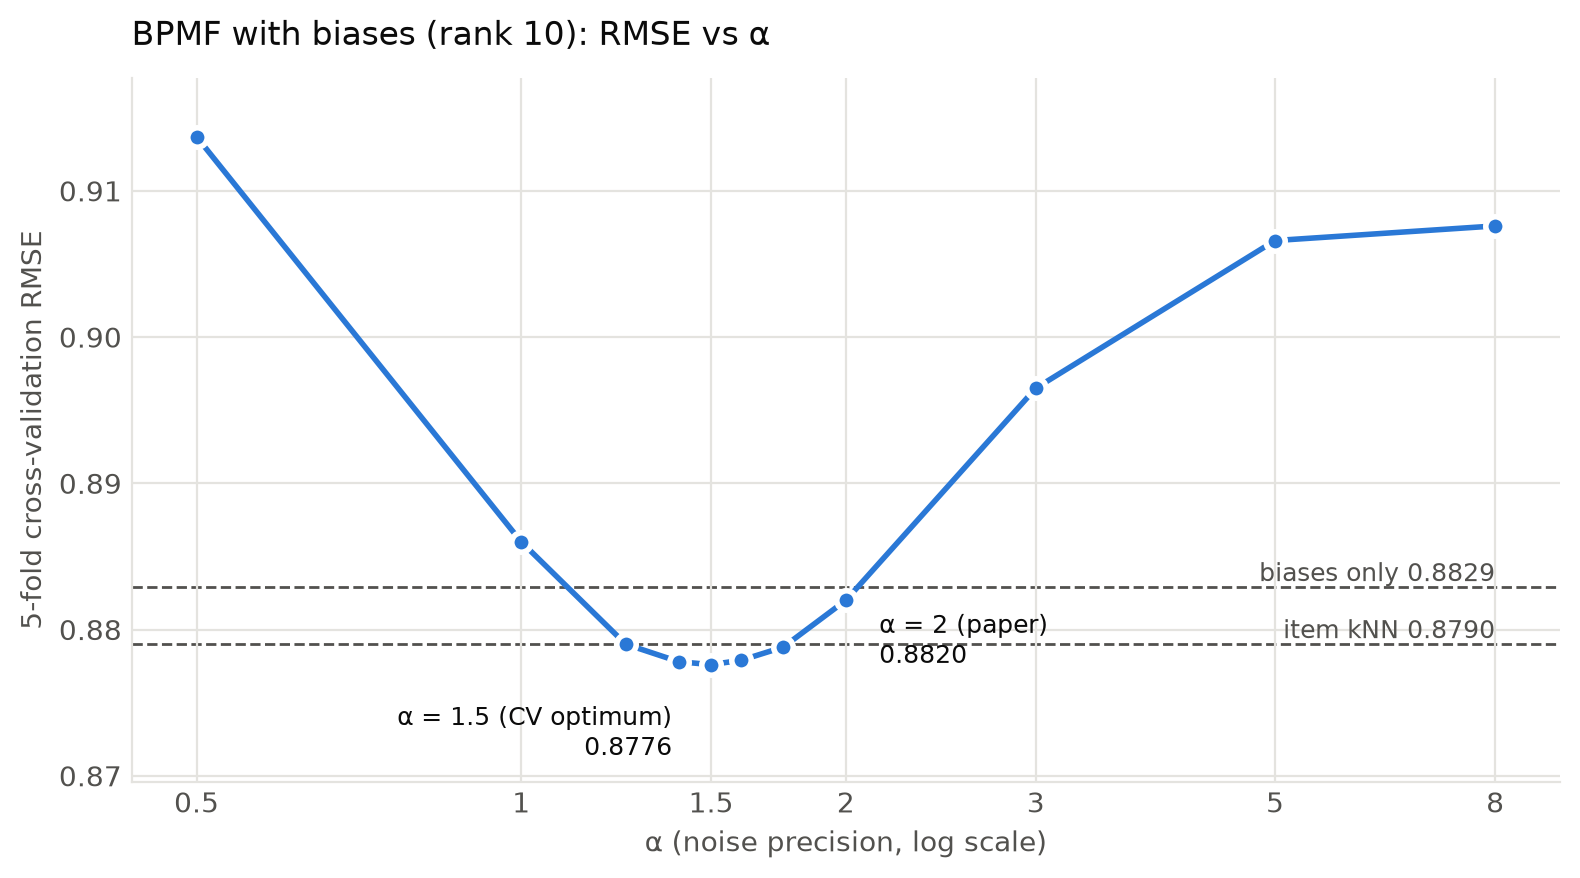
\includegraphics[width=\columnwidth]{bpmf_alpha.png}
\caption{BPMF with biases, rank 10: 5-fold CV RMSE on the train set, used to choose the noise precision
$\alpha$.}
\label{fig:alpha}
\end{figure}

The noise precision acts as a regularization strength, and Figure~\ref{fig:alpha} shows how we chose it on the
train set. With the paper's $\alpha = 2$ (noise standard deviation $0.71$), BPMF only matches the biases there.
The optimum $\alpha = 1.5$ (standard deviation $0.82$) is closer to the error level actually reached, and on
train $\cup$ test it is better than $\alpha = 2$ by $0.0026$. We also sampled $\alpha$ in the Gibbs chain, with a
conjugate $\mathrm{Gamma}(1,1)$ prior. It does not help ($+0.0014$, better on 1 fold of 5), and $\alpha$ drifts
from $1.6$ to $2.4$: it is fitted to the training residuals of the current sample, which shrink as the chain
overfits. A fixed $\alpha$ acts as a regularization that the sampled one loses.

%% ================================================================ 4
\section{Bayesian factorization machines}

A factorization machine~\cite{fm} predicts from a sparse feature vector $x$:
\[
\rhat(x) = w_0 + \sum_j w_j x_j + \sum_{j<l} \langle v_j, v_l\rangle\, x_j x_l .
\]
With $x$ equal to the one-hot of $u$ concatenated with the one-hot of $i$, this is exactly BPMF with biases.
The Bayesian FM~\cite{bfm} keeps the same Gibbs scheme and differs from BPMF in three ways: any feature can
enter $x$; each feature group (users, movies, genres, \dots) has its own Gaussian prior with Normal-Gamma
hyperpriors on its mean and diagonal precision, instead of a full Wishart; and $\alpha$ is sampled.

Following~\cite{baselines}, our feature vector adds two kinds of information to the two one-hot blocks. The
implicit feedback puts in the user block the movies rated by $u$, each with value $|\Omega_u|^{-1/2}$ as in
SVD++~\cite{koren}, and in the movie block the users who rated $i$, with value $|\Omega_i|^{-1/2}$. These sets
are built from the training ratings only. The side information is the genres (multi-hot) and the release
decade (one-hot) of the movie. The genre file first provided was aligned with only 648 of the 4980 columns;
with it, the full model is worse by $0.016$ on every fold.

\subsection{Features, rank and chains}\label{sec:fm-results}
Without features, the FM performs as BPMF ($0.8465$ against $0.8479$, $p = 0.41$). Both groups of features
help, the genres most: over the FM without features, the implicit feedback gains $0.0125$ and the genres
$0.0275$, on every fold. With the genres already in, the implicit feedback adds only $0.0019$, on 4 folds of 5,
which is not significant ($p = 0.17$): the two groups carry overlapping information. We keep both. The genres
help most where the ratings are fewest, since they describe a movie that has no neighbours.

On the train set alone, ranks 5 and 20 are indistinguishable ($0.8472$ and $0.8478$). On train $\cup$ test,
rank 20 is clearly better ($0.8203$ for rank 5, $0.8171$ for 20, $0.8168$ for 30, $0.8186$ for 40). More
ratings support more latent dimensions, so hyperparameters tuned on half the data are biased towards small
models; this is why we evaluate on the union. We keep rank 20 and 238 iterations.

The FM samples $\alpha$, and it underestimates the noise: the noise standard deviation $\alpha^{-1/2}$ settles
near $0.55$, while the actual error of the averaged prediction is $0.82$. The model believes the training
ratings more than it should, so a single sample drifts towards overfitting (its RMSE rises from $0.87$ to
$0.97$), and we stop after the number of iterations that minimizes the CV error. Independent chains explore
different regions of the posterior. Averaging the posterior means of 2, 3, 5 and 10 chains gives $0.8141$,
$0.8125$, $0.8117$ and $0.8113$. We keep 5 chains, which gain $0.0054$ over one on every fold; the next 5
bring only $0.0004$.

\begin{figure*}[t]
\centering
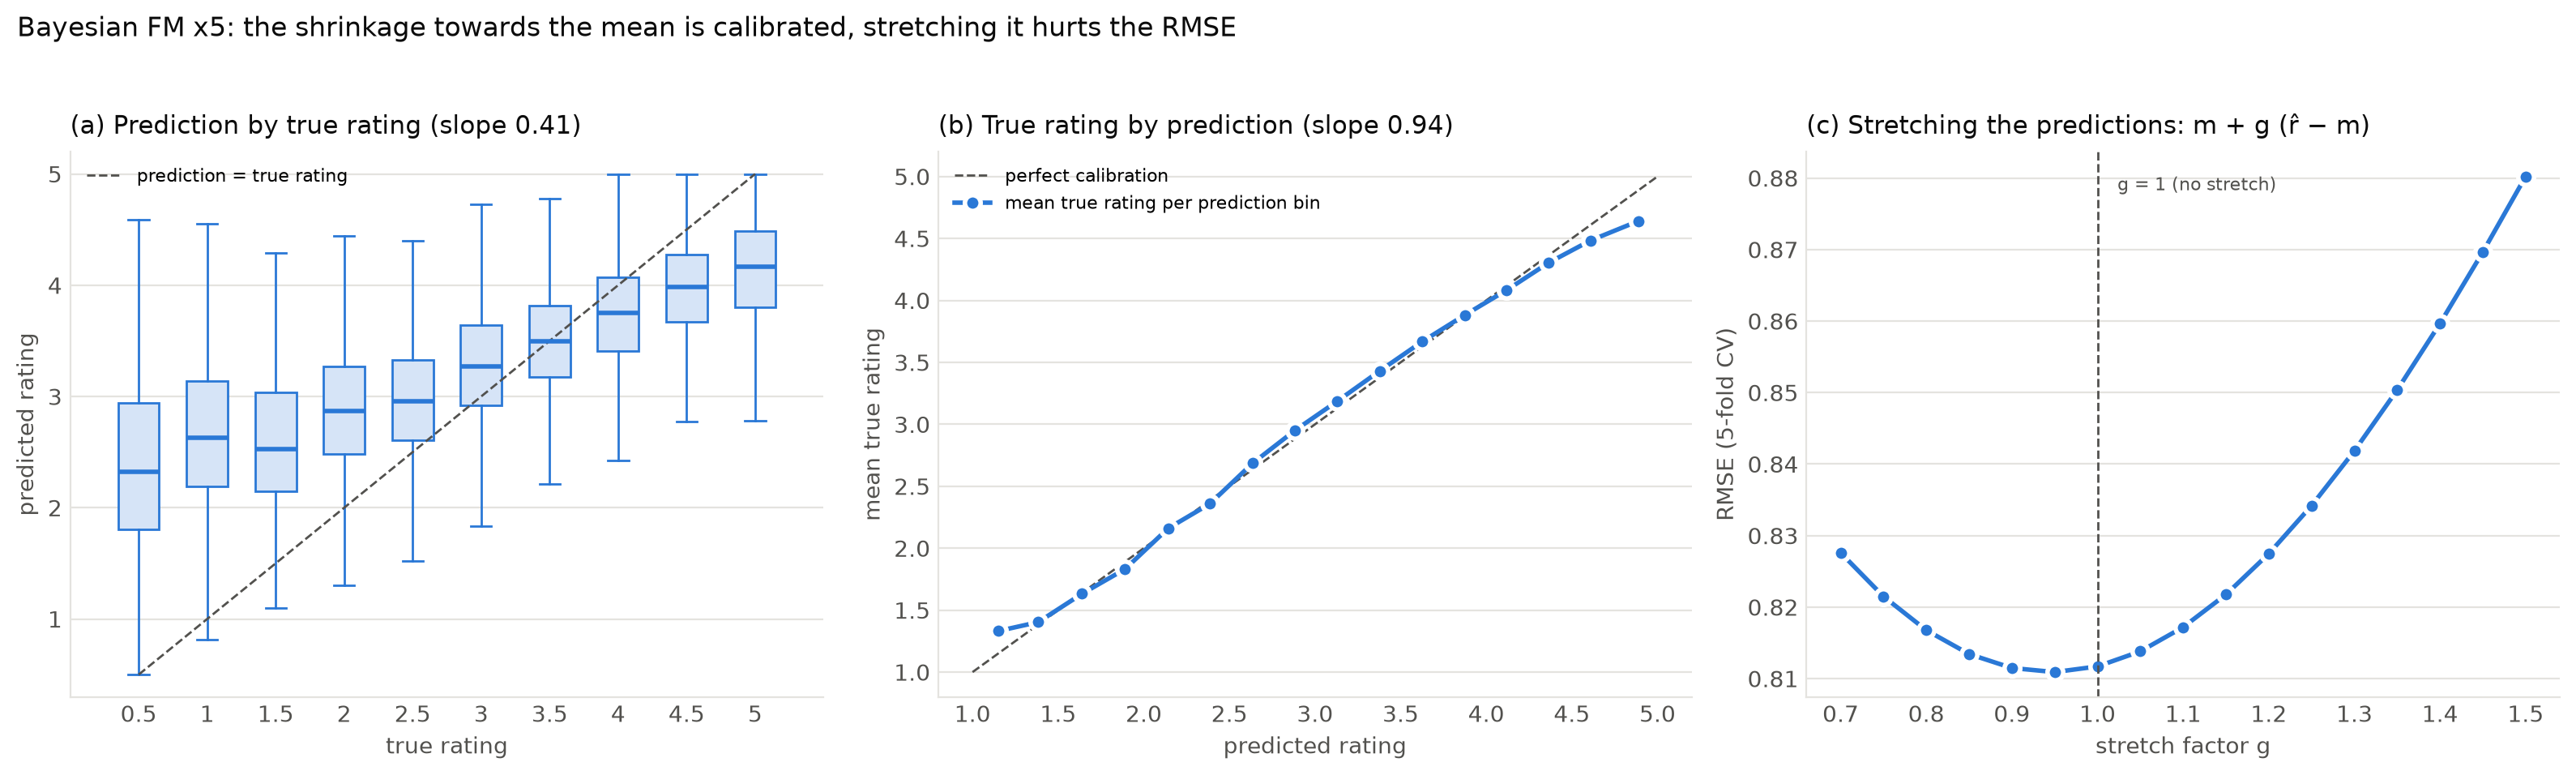
\includegraphics[width=\textwidth]{1a_extremes_calibration.png}
\caption{Bayesian FM $\times 5$, out-of-fold predictions on train $\cup$ test. (a) Prediction against the true
rating. (b) Mean true rating by prediction bin (calibration). (c) CV RMSE after stretching the predictions by $g$.}
\label{fig:calib}
\end{figure*}

\subsection{Extreme ratings are pulled to the mean, as RMSE requires}\label{sec:extremes}
We now analyse the out-of-fold predictions of the FM $\times 5$ alone. The slope of the predictions against
the true ratings is only $0.41$, and ratings of $0.5$ are predicted $2.4$ on average (Figure~\ref{fig:calib}a).
This is the expected behaviour of the RMSE-optimal predictor. The minimizer of $\E[(r - f(x))^2]$ is
$f^*(x) = \E[r \mid x]$, and nothing in the features $x$ (identities, past ratings, genres) announces that a
user will give $0.5$ to a movie the model expects them to like. $\E[r\mid x]$ averages the possible ratings and
lands in between. The other direction confirms it: the mean true rating at a given prediction follows the
diagonal with slope $0.94$ (Figure~\ref{fig:calib}b), so the model is calibrated,
$\E[r \mid \rhat] \approx \rhat$. For a calibrated predictor $\Cov(\rhat, r - \rhat) = 0$, hence the slope of
$\rhat$ on $r$ is
\[
\frac{\Cov(\rhat, r)}{\Var(r)} = \frac{\Var(\rhat)}{\Var(r)} = 1 - \frac{\mathrm{MSE}}{\Var(r)} .
\]
With $\Var(r) = 1.071$ and $\mathrm{MSE} = 0.659$ this gives $0.385$, close to the measured $0.41$. The
shrinkage towards the mean is the variance the model cannot explain; it decreases only with more information,
not with a correction of the outputs. Figure~\ref{fig:calib}c tests the correction anyway: stretching the
predictions around their mean $m$, $\rhat' = m + g(\rhat - m)$, degrades the RMSE ($0.842$ for $g = 1.3$).
The best factor is $g = 0.95$ ($0.8109$), because the FM is slightly over-dispersed (calibration slope
$0.94 < 1$); the linear stack applies this correction automatically.

\subsection{Users with spread-out ratings and user normalization}
Users whose ratings have a standard deviation above 1 account for $31\%$ of the ratings and $46\%$ of the
squared error (Figure~\ref{fig:segments}a). The FM has a single noise level $\alpha^{-1}$ for all users, so a
user who uses the whole scale and a user who only gives 3.5 to 4.5 are fitted with the same confidence. We fit
the FM on normalized ratings $z_{ui} = (r_{ui} - m_u)/s_u$ and map back with $\rhat_{ui} = m_u + s_u \hat z_{ui}$,
where the user mean and standard deviation are shrunk towards the global ones with $\kappa = 20$
pseudo-ratings:
\begin{gather*}
m_u = \frac{\sum_{i\in\Omega_u} r_{ui} + \kappa\mu}{|\Omega_u| + \kappa},\\
s_u^2 = \frac{\sum_{i\in\Omega_u} (r_{ui} - m_u)^2 + \kappa\sigma^2}{|\Omega_u| + \kappa}.
\end{gather*}
The normalization is computed on the training ratings of each fold, so the evaluation set is never used.
The CV RMSE of the FM $\times 5$ goes from $0.8117$ to $0.8049$ ($-0.0068$, on 5 folds out of 5). Every
segment gains, the most spread-out users the most ($-0.015$ for a standard deviation $\ge 1.2$), and so do the
least spread-out ones ($-0.009$), whose narrow scale is now respected.

\begin{figure*}[t]
\centering
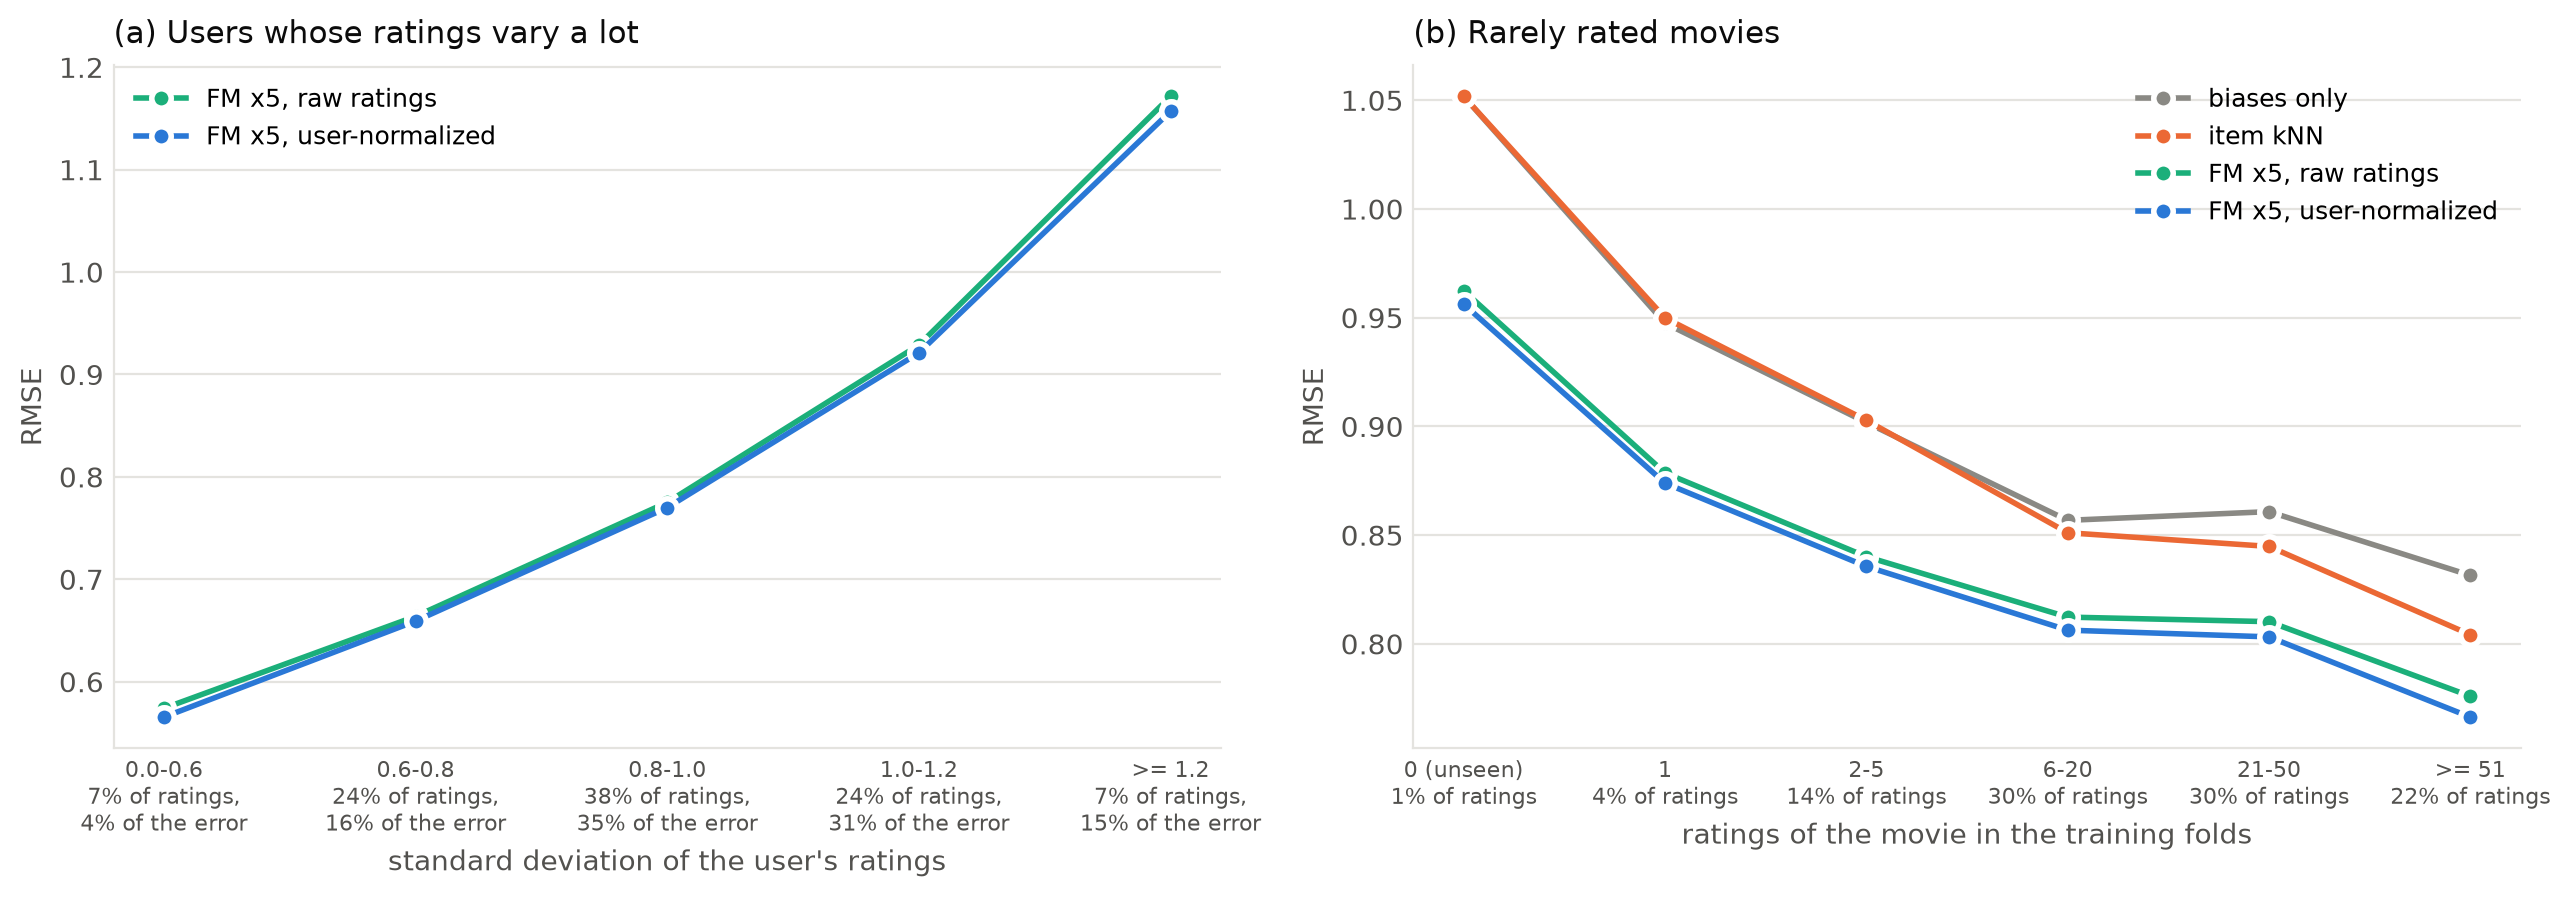
\includegraphics[width=\textwidth]{1bc_users_and_movies.png}
\caption{Out-of-fold RMSE by segment. (a) By standard deviation of the user's ratings, FM $\times 5$ on raw and
normalized ratings. (b) By number of training ratings of the movie: biases, item kNN, FM raw and normalized.}
\label{fig:segments}
\end{figure*}

\begin{figure*}[t]
\centering
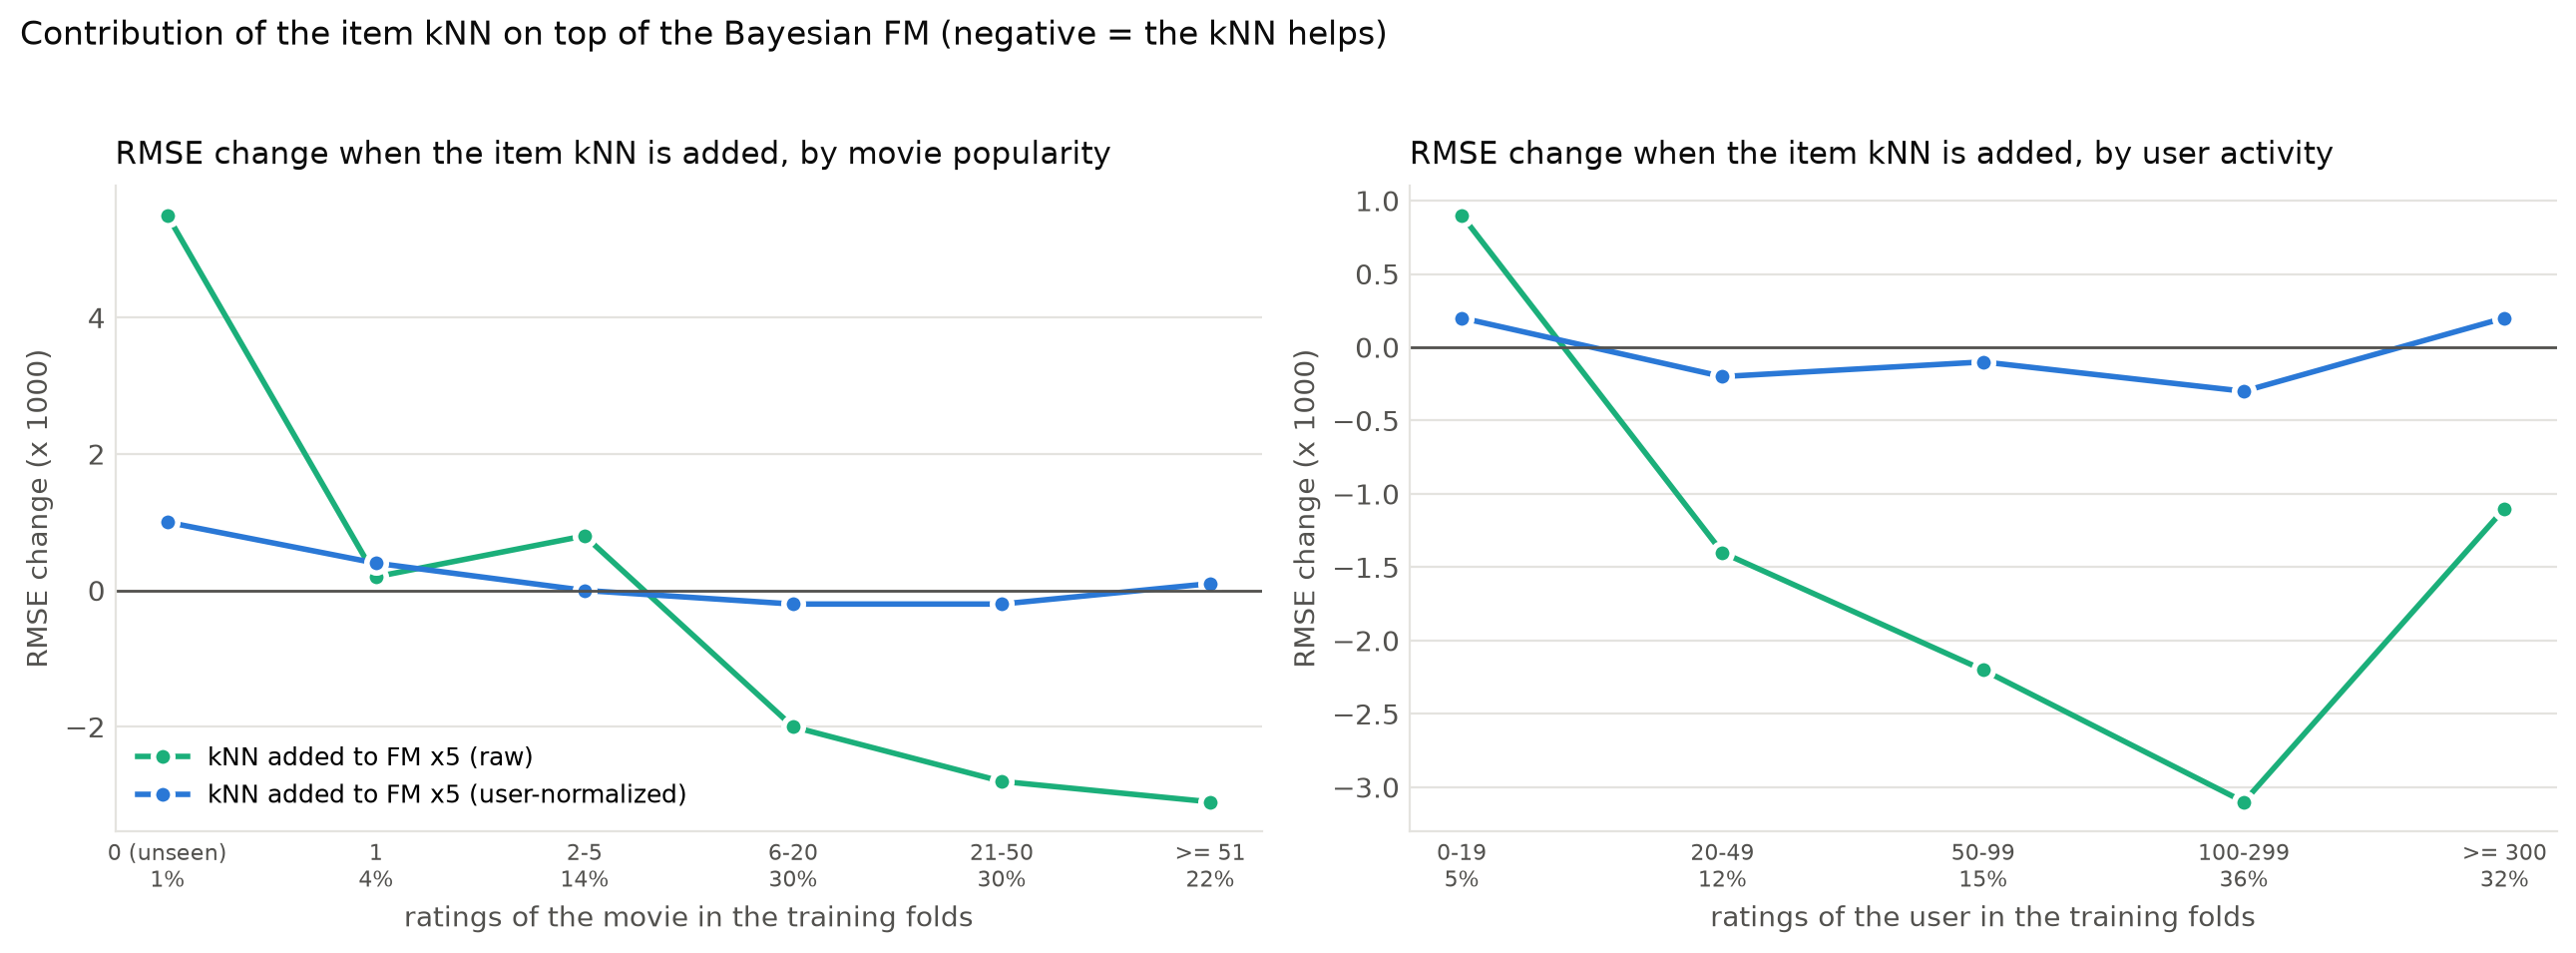
\includegraphics[width=\textwidth]{2_knn_contribution.png}
\caption{RMSE change ($\times 1000$) when the item kNN is added to the FM $\times 5$ in a linear stack, by
segment.}
\label{fig:knn}
\end{figure*}

\subsection{Rarely rated movies}
$18\%$ of the evaluation ratings concern a movie with at most 5 training ratings (Figure~\ref{fig:segments}b).
There, the item kNN is no better than the biases because it has no neighbours to average. The FM is $0.06$ to
$0.09$ better than both, thanks to the genres and to the implicit feedback (who rated the movie). These movies
remain the hardest segment ($0.96$ for unseen movies, against $0.77$ above 50 ratings), and normalization
helps them only slightly.

\subsection{Combining the FM with the item kNN}
The two models use different information, latent factors and side features on one side, local co-ratings on
the other. We combined them linearly,
$\rhat = w_0 + w_{\text{FM}}\rhat^{\text{FM}} + w_{\text{kNN}}\rhat^{\text{kNN}}$, with weights fitted by
least squares on out-of-fold predictions and evaluated on other folds (Table~\ref{tab:stack}).

\begin{table}[h]
\centering\footnotesize
\setlength{\tabcolsep}{3pt}
\begin{tabular}{@{}lcc@{}}
\toprule
 & raw FM & normalized FM \\
\midrule
$w_{\text{FM}}$ / $w_{\text{kNN}}$        & 0.821 / 0.161 & 0.981 / $-0.006$ \\
RMSE, FM $\to$ stack                      & $0.8117 \to 0.8098$ & $0.8049 \to 0.8048$ \\
Error correlation                         & 0.926 & 0.942 \\
kNN share of $\Var(\rhat)$                & $2.6\%$ & $0\%$ \\
\bottomrule
\end{tabular}
\caption{Linear stack of the FM $\times 5$ and the item kNN.}
\label{tab:stack}
\end{table}

With the raw FM, the kNN brings $-0.0019$ on every fold, and only where it has neighbours
(Figure~\ref{fig:knn}): $-0.003$ on movies with more than 20 ratings and on users with 100 to 300 ratings,
while it degrades unseen movies ($+0.0055$), where it only repeats the biases. The errors of the two models are
correlated at $0.93$: they fail on the same ratings, which we expect to be the unpredictable extremes of
Section~\ref{sec:extremes}. After normalization the kNN weight is zero, as the normalization already corrects
what the kNN corrected. The raw FM with the kNN was our submission 3 ($0.801$ on the platform).

\subsection{Gradient boosting on the stack residual}
A linear stack gives the kNN the same weight everywhere, while it is only useful on popular movies. We fit a
gradient-boosted tree model~\cite{friedman} (200 trees, 15 leaves, at least 200 ratings per leaf) on the
residual of the linear stack of the normalized FM, the raw FM and the kNN. Its features are the base
predictions, the disagreement between the 5 chains, the user and movie counts, means and standard deviations,
the user's share of half-star ratings, the genres and the decade. Fitted and evaluated across folds, it brings
the CV RMSE to $0.8023$ ($-0.0025$ on top of the linear stack, on 5 folds out of 5, $p = 0.002$). This is our
final submission; with the observed gap between CV and platform, we expect about $0.795$.

%% ================================================================ 5
\section{Discussion}

The gains came from averaging over the posterior (BPMF, Bayesian FM, several chains), from side information
on the movies and from user normalization, each holding on every fold. The methods of the course gain at most
$0.012$ over the biases, stretching the predictions cannot work under RMSE, and the item kNN adds almost
nothing to a normalized FM in a linear combination.

Three limitations remain. The stacking models are trained on out-of-fold predictions of models fitted on
$80\%$ of train $\cup$ test, while the submitted base models are fitted on $100\%$, so their predictions are
slightly sharper than those the stack learnt from. The rank and the number of iterations of the FM were chosen
on the folds that measure them, which biases its score slightly downwards. The gap between CV and platform
($\approx 0.009$) has been stable over two submissions only.

At $1\%$ density, the bottleneck is information, not the optimizer: ALS and gradient descent reach the same
minimum, while integrating over the uncertainty and adding information (genres, implicit feedback, per-user
scale) each brought a gain. Hyperparameters must be tuned at the data size of the final fit.

%% ================================================================ 6
\section{Conclusion}

On a matrix this sparse, the methods of the course quickly reach a ceiling set by the bias model. The steps
that moved the error further address the lack of data per movie and per user. Measured on the same folds,
our path reads:
\begin{center}\small
\begin{tabular}{@{}lc@{}}
\toprule
Step & CV RMSE \\
\midrule
Regularized biases                    & 0.8642 \\
Best course method (item kNN)         & 0.8523 \\
Posterior averaging (BPMF)            & 0.8479 \\
Genres in a Bayesian FM               & 0.8190 \\
Implicit feedback                     & 0.8171 \\
Five chains                           & 0.8117 \\
User normalization                    & 0.8049 \\
Stack with item kNN and boosting      & \textbf{0.8023} \\
\bottomrule
\end{tabular}
\end{center}

{\small
\begin{thebibliography}{9}
\setlength{\itemsep}{1pt}
\setlength{\parsep}{0pt}
\bibitem{bpmf} R. Salakhutdinov and A. Mnih. Bayesian probabilistic matrix factorization using Markov chain
Monte Carlo. ICML, 2008.
\bibitem{koren} Y. Koren. Factorization meets the neighborhood: a multifaceted collaborative filtering model.
KDD, 2008.
\bibitem{fm} S. Rendle. Factorization machines. ICDM, 2010.
\bibitem{bfm} C. Freudenthaler, L. Schmidt-Thieme and S. Rendle. Bayesian factorization machines. NIPS Workshop
on Sparse Representation and Low-rank Approximation, 2011.
\bibitem{baselines} S. Rendle, L. Zhang and Y. Koren. On the difficulty of evaluating baselines: a study on
recommender systems. arXiv:1905.01395, 2019.
\bibitem{nadeau} C. Nadeau and Y. Bengio. Inference for the generalization error. Machine Learning, 52(3), 2003.
\bibitem{friedman} J. H. Friedman. Greedy function approximation: a gradient boosting machine. Annals of
Statistics, 29(5), 2001.
\bibitem{myfm} T. Ohtsuki. myFM: Bayesian factorization machines in Python/C++.
\url{https://github.com/tohtsky/myFM}.
\end{thebibliography}
}

\end{document}
